%versi 3 (22-07-2020)
\chapter{Landasan Teori}
\label{chap:landasan_teori}

\section{Point of Interest}
\label{sec:poi}

\textit{Point of Interest} (POI) adalah sebuah lokasi geografis.

\section{Object Instance Recognition}
\label{sec:oir}

\textit{Object Instance Recognition} (OIR) adalah teknik pengenalan objek spesifik.

\section{SIFT (Speeded Up Robust Feature)}
\label{sec:sift}

SIFT adalah salah satu metode pencarian fitur lokal. Fitur lokal yang dihasilkan SIFT bersifat invarian terhadap rotasi, perubahan skala, dan translasi pada gambar. Sifat invarian ini berarti fitur lokal yang sama pada gambar yang telah di rotasi, diubah skalanya, atau di translasi akan tetap memiliki ciri yang mirip. Setiap fitur lokal akan memiliki sebuah vektor yang mendeskripsikan daerah area fitur lokal tersebut, vektor ini biasa disebut sebagai deskriptor. Vektor deksriptor SIFT berbentuk vektor bilangan bulat yang memiliki 128 elemen. Tahap pencarian fitur lokal pada SIFT dibagi menjadi 4 langkah sebagai berikut.

\subsection{Pencarian Extrema}
Pada tahap ini akan dicari \textit{pixel-pixel} pada gambar yang merupakan \textit{corner} atau biasa disebut \textit{keypoint}. \textit{Keypoint} pada SIFT dicari dengan memeriksa \textit{pixel-pixel} pada gambar hasil turunan kedua Gaussian. 

Pencarian \textit{keypoint} ini dilakukan dengan memanfaatkan sifat dari \textit{Matrix} Konvolusi Gaussian. \textit{Matrix} Konvolusi Gaussian merupakan \textit{matrix} yang memiliki sifat distribusi Gaussian, di mana titik tengah \textit{matrix} memiliki nilai yang tinggi dan nilai-nilai di sekitarnya berkurang semakin mendekati tepi \textit{matrix}. Seperti ditunjukkan pada Gambar~\ref{fig:gaussian_function}. 
\begin{figure}[H]
	\begin{subfigure}[b]{.5\textwidth}
		\centering
		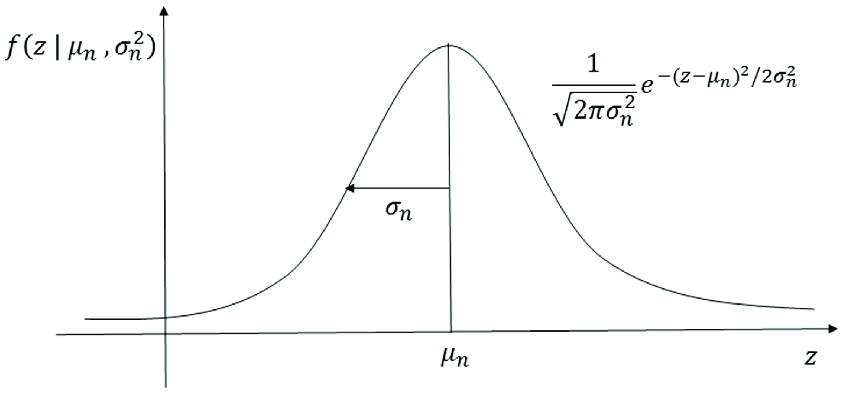
\includegraphics[width=0.9\linewidth]{gaussian_curve_s.png}
		\caption{}
		\label{subfig:gaussian_curve}
	\end{subfigure}%
	\begin{subfigure}[b]{.5\textwidth}
		\centering
		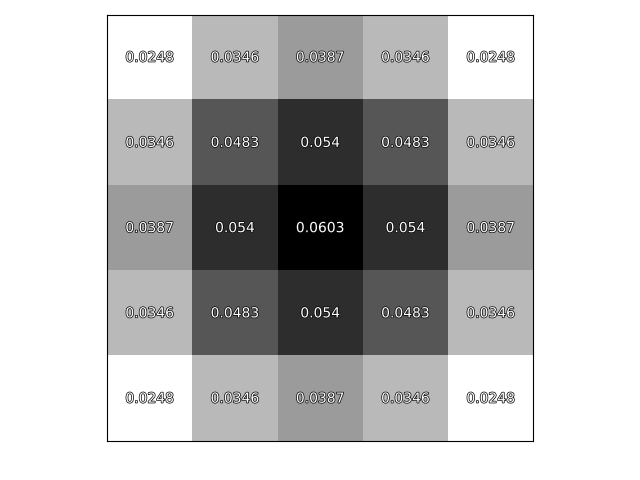
\includegraphics[width=0.9\linewidth]{gaussian_matrix_3.png}
		\caption{}
		\label{subfig:gaussian_matrix}
	\end{subfigure}
	\caption{Kurva Gaussian dan bentuk representasi \textit{matrix}-nya.}
	\label{fig:gaussian_function}
\end{figure}

Pada fungsi Gaussian tingkat penyebaran data dapat diatur dengan mengubah parameter $\sigma$ yang mengatur nilai standar deviasi. Gambar~\ref{subfig:gaussian_curve} menunjukkan bagaimana nilai $\sigma$ mengatur bagaimana data tersebar dari \textit{mean}, di mana semakin tinggi nilai $\sigma$ maka data akan semakin menyebar. Nilai yang semakin menyebar menyebabkan perbedaan nilai antar titik semakin kecil. Efeknya pada \textit{matrix} dapat dilihat pada Gambar~\ref{fig:gaussian_sigma}. Nilai $\sigma$ yang tinggi menyebabkan kurva semakin melebar dan pada \textit{matrix} selisih nilai antar titik menjadi semakin kecil.

\begin{figure}[H]
	\begin{subfigure}[b]{.5\textwidth}
		\centering
		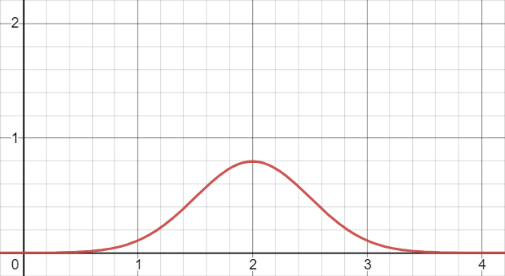
\includegraphics[width=0.9\linewidth]{gaussian_curve_1.png}
		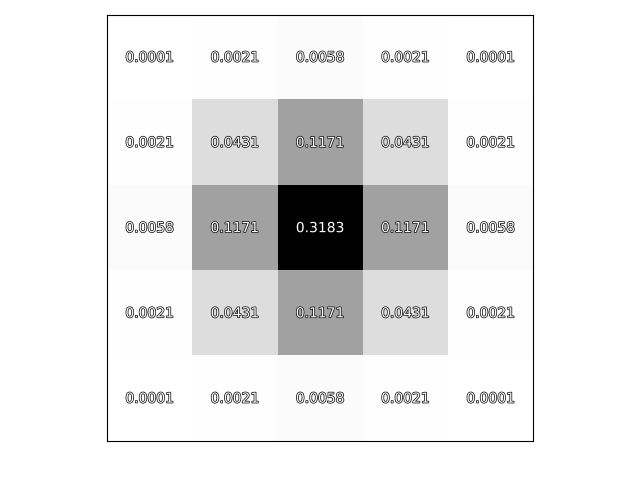
\includegraphics[width=0.9\linewidth]{gaussian_matrix_1.png}
		\caption{$\sigma=1$}
		\label{subfig:gaussian_sigma1}
	\end{subfigure}%
	\begin{subfigure}[b]{.5\textwidth}
		\centering
		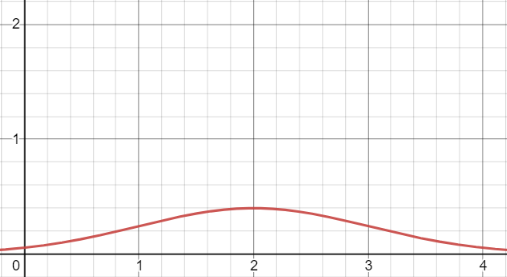
\includegraphics[width=0.9\linewidth]{gaussian_curve_2.png}
		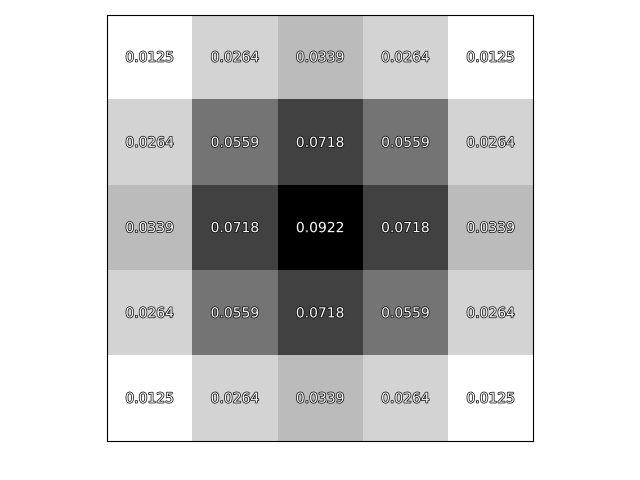
\includegraphics[width=0.9\linewidth]{gaussian_matrix_2.png}
		\caption{$\sigma=2$}
		\label{subfig:gaussian_sigma2}
	\end{subfigure}
	\caption{Kurva dan \textit{matrix} Gaussian pada nilai $\sigma$ yang berbeda.}
	\label{fig:gaussian_sigma}
\end{figure}

\textit{Matrix} Konvolusi Gaussian ketika diaplikasikan pada gambar akan menyebabkan perubahan nilai tiap \textit{pixel} pada gambar. Nilai dari setiap \textit{pixel} akan menjadi mirip dengan \textit{pixel} tetangga di dekatnya. Perubahan nilai \textit{pixel} akan paling berpengaruh pada daerah dengan perubahan nilai \textit{pixel} yang tinggi. Tingkat perubahan nilai dipengaruhi oleh nilai $\sigma$ yang digunakan, nilai $\sigma$ yang tinggi akan menyebabkan nilai \textit{pixel} yang berdekatan semakin mirip---perubahan nilai \textit{pixel} pada daerah tersebut semakin mengecil. Jika dilihat pada gambar, maka gambar hasil konvolusi akan terlihat kabur (\textit{blur}). Nilai $\sigma$ menentukan tingkat \textit{blur} gambar.

\begin{figure}[H]
	\centering
	\begin{subfigure}[b]{.33\textwidth}
		\centering
		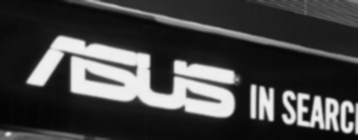
\includegraphics[width=0.9\linewidth]{1.0_asus_logo2.jpeg}
		\caption{$\sigma=1.0$}
		\label{subfig:asus_sigma1.0}
	\end{subfigure}%
	\begin{subfigure}[b]{.33\textwidth}
		\centering
		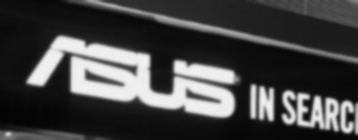
\includegraphics[width=0.9\linewidth]{1.4_asus_logo2.jpeg}
		\caption{$\sigma=1.4$}
		\label{subfig:asus_sigma1.4}
	\end{subfigure}
	\begin{subfigure}[b]{.33\textwidth}
		\centering
		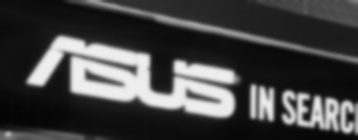
\includegraphics[width=0.9\linewidth]{1.8_asus_logo2.jpeg}
		\caption{$\sigma=1.8$}
		\label{subfig:asus_sigma1.8}
	\end{subfigure}
	\caption{Efek nilai $\sigma$ pada hasil gambar konvolusi.}
	\label{fig:asus_konv}
\end{figure}

Perubahan nilai $\sigma$ pada \textit{matrix} konvolusi serta efeknya pada gambar akan dimanfaatkan untuk menghitung \textit{Difference of Gaussian} (DoG). DoG merupakan hasil turunan kedua Gaussian pada gambar. Gambar DoG dapat diperoleh dengan menghitung perbedaan nilai tiap \textit{pixel} dari dua gambar yang telah dikonvolusi oleh \textit{matrix} Gaussian dengan nilai $\sigma$ yang berbeda. Perbedaan nilai untuk DoG dihitung dengan mengurangi setiap \textit{pixel} pada gambar konvolusi yang memiliki nilai $\sigma$ yang lebih kecil, dengan setiap \textit{pixel} pada posisi yang sama pada gambar konvolusi yang memiliki nilai $\sigma$ yang lebih besar. Ilustrasi dapat dilihat pada Gambar~\ref{fig:dog_asus}. 
\begin{figure}[t]
	\centering
	\includegraphics[width=\linewidth]{asus_dog.png}
	\caption{Operasi DoG pada gambar}
	\label{fig:dog_asus}
\end{figure} 

Metode SIFT mencari \textit{keypoint} dengan memanfaatkan konsep DoG. Sebuah gambar akan dikonvolusi dengan \textit{matrix} Gaussian beberapa kali dengan nilai $\sigma$ yang berbeda. Setelah didapatkan beberapa gambar maka akan dihitung DoG untuk setiap gambar yang nilai $\sigma$-nya bersebelahan (Gambar~\ref{fig:dog_scales}), dari hasil DoG tersebut yang akan digunakan untuk mencari \textit{keypoint}. Untuk setiap gambar DoG akan ditentukan \textit{pixel} mana saja yang merupakan \textit{keypoint} dengan mencari \textit{pixel} yang merupakan \textit{extrema}. Sebuah \textit{pixel} merupakan \textit{extrema} jika nilai pixel tersebut lebih besar dari seluruh 26 \textit{pixel} di sekitarnya atau lebih kecil dari seluruhnya. Ke-26 \textit{pixel} tersebut merupakan 8 \textit{pixel} yang mengelilingi, 9 \textit{pixel} pada posisi yang sama dari gambar di atasnya, dan juga 9 \textit{pixel} pada posisi yang sama dari gambar di bawahnya.
\begin{figure}[H]
	\centering
	\includegraphics[width=0.7\linewidth]{dog_scales.png}
	\caption{Penggunaan DoG pada SIFT}
	\label{fig:dog_scales}
\end{figure} 

\subsection{Penentuan Skala}
Pada tahap sebelumnya sudah didapatkan \textit{keypoint-keypoint} dalam gambar. Agar \textit{keypoint} dapat invarian terhadap skala, \textit{keypoint} perlu untuk dapat tetap terdeteksi walaupun ukuran gambar berubah. Untuk setiap \textit{keypoint} perlu untuk dicari skala terkecil di mana \textit{keypoint} tersebut dapat terdeteksi. Untuk mencapai ini SIFT menggunakan lanjutan dari metode pada Gambar~\ref{fig:dog_scales}. Saat nilai $\sigma$ sudah mencapai 2 kali dari nilai awalnya---atau yang disebut sudah menyelesaikan satu oktaf---maka proses akan dilanjutkan ke oktaf berikutnya, gambar akan diperkecil (\textit{downsample}) ukuran menjadi setengahnya dan proses konvolusi diulang lagi (Gambar~\ref{fig:oktaf}). Untuk oktaf baru tersebut akan dihitung DoG-nya dan dicari \textit{extrema}-nya. Untuk setiap \textit{keypoint} akan dicatat oktaf terbesar (ukuran gambar terkecil) di mana gambar \textit{keypoint} tersebut tetap ditemukan. 
\begin{figure}
	\centering
	\includegraphics[width=0.7\linewidth]{oktaf.png}
	\caption{Oktaf pada proses konvolusi SIFT}
	\label{fig:oktaf}
\end{figure}

\subsection{Penentuan Orientasi}
Untuk dapat invarian terhadap rotasi gambar, setiap \textit{keypoint} perlu memiliki orientasi yang konsisten. Untuk mendapatkan orientasi yang sama pada setiap rotasi gambar, orientasi perlu ditentukan dari atribut yang akan selalu sama bagaimanapun gambar dirotasi. Untuk itu orientasi \textit{keypoint} ditentukan dengan menggunakan orientasi yang dominan dari \textit{pixel-pixel} di sekitar \textit{keypoint}. Luas daerah yang digunakan untuk mendapat orientasi ditentukan oleh skala dari \textit{keypoint}. 

Penentuan orientasi yang dominan dihitung dengan menggunakan \textit{magnitude}, $m(x,y)$, dan orientasi, $\theta(x,y)$, dari \textit{pixel-pixel} dengan menggunakan rumus berikut, $L(x,y)$ merupakan gambar hasil konvolusi:
\[ 
m(x,y)=\sqrt{(L(x+1,y)-L(x-1,y))^{2}+L(x,y+1)-L(x,y+1))^{2}} 
\]
\[
\theta(x,y)=\tan^{-1}((L(x,y+1)-L(x,y-1))/(L(x+1,y)-L(x-1,y)))
\]
Setiap \textit{pixel} akan dihitung orientasi dan \textit{magnitude}-nya. \textit{Magnitude} akan digunakan sebagai bobot dari \textit{pixel} tersebut. Selain \textit{magnitude}, bobot sebuah \textit{pixel} juga dipengaruhi oleh \textit{Gaussian Weighting}. \textit{Pixel} yang posisinya dekat dengan titik pusat (pusat \textit{keypoint}) akan memiliki bobot yang lebih tinggi dibanding yang lokasinya jauh. 

Setelah setiap \textit{pixel} sudah dihitung orientasi dan bobotnya---menggunakan \textit{magnitude} dan \textit{Gaussian Weighting}---nilai bobot tersebut akan dimasukkan ke dalam histogram berdasarkan orientasinya. Histogram yang digunakan memiliki 36 bin yang masing-masing mewakili 10 derajat orientasi. Ilustrasi dapat dilihat pada Gambar~\ref{fig:hist_orientasi}.
\begin{figure}
	\centering
	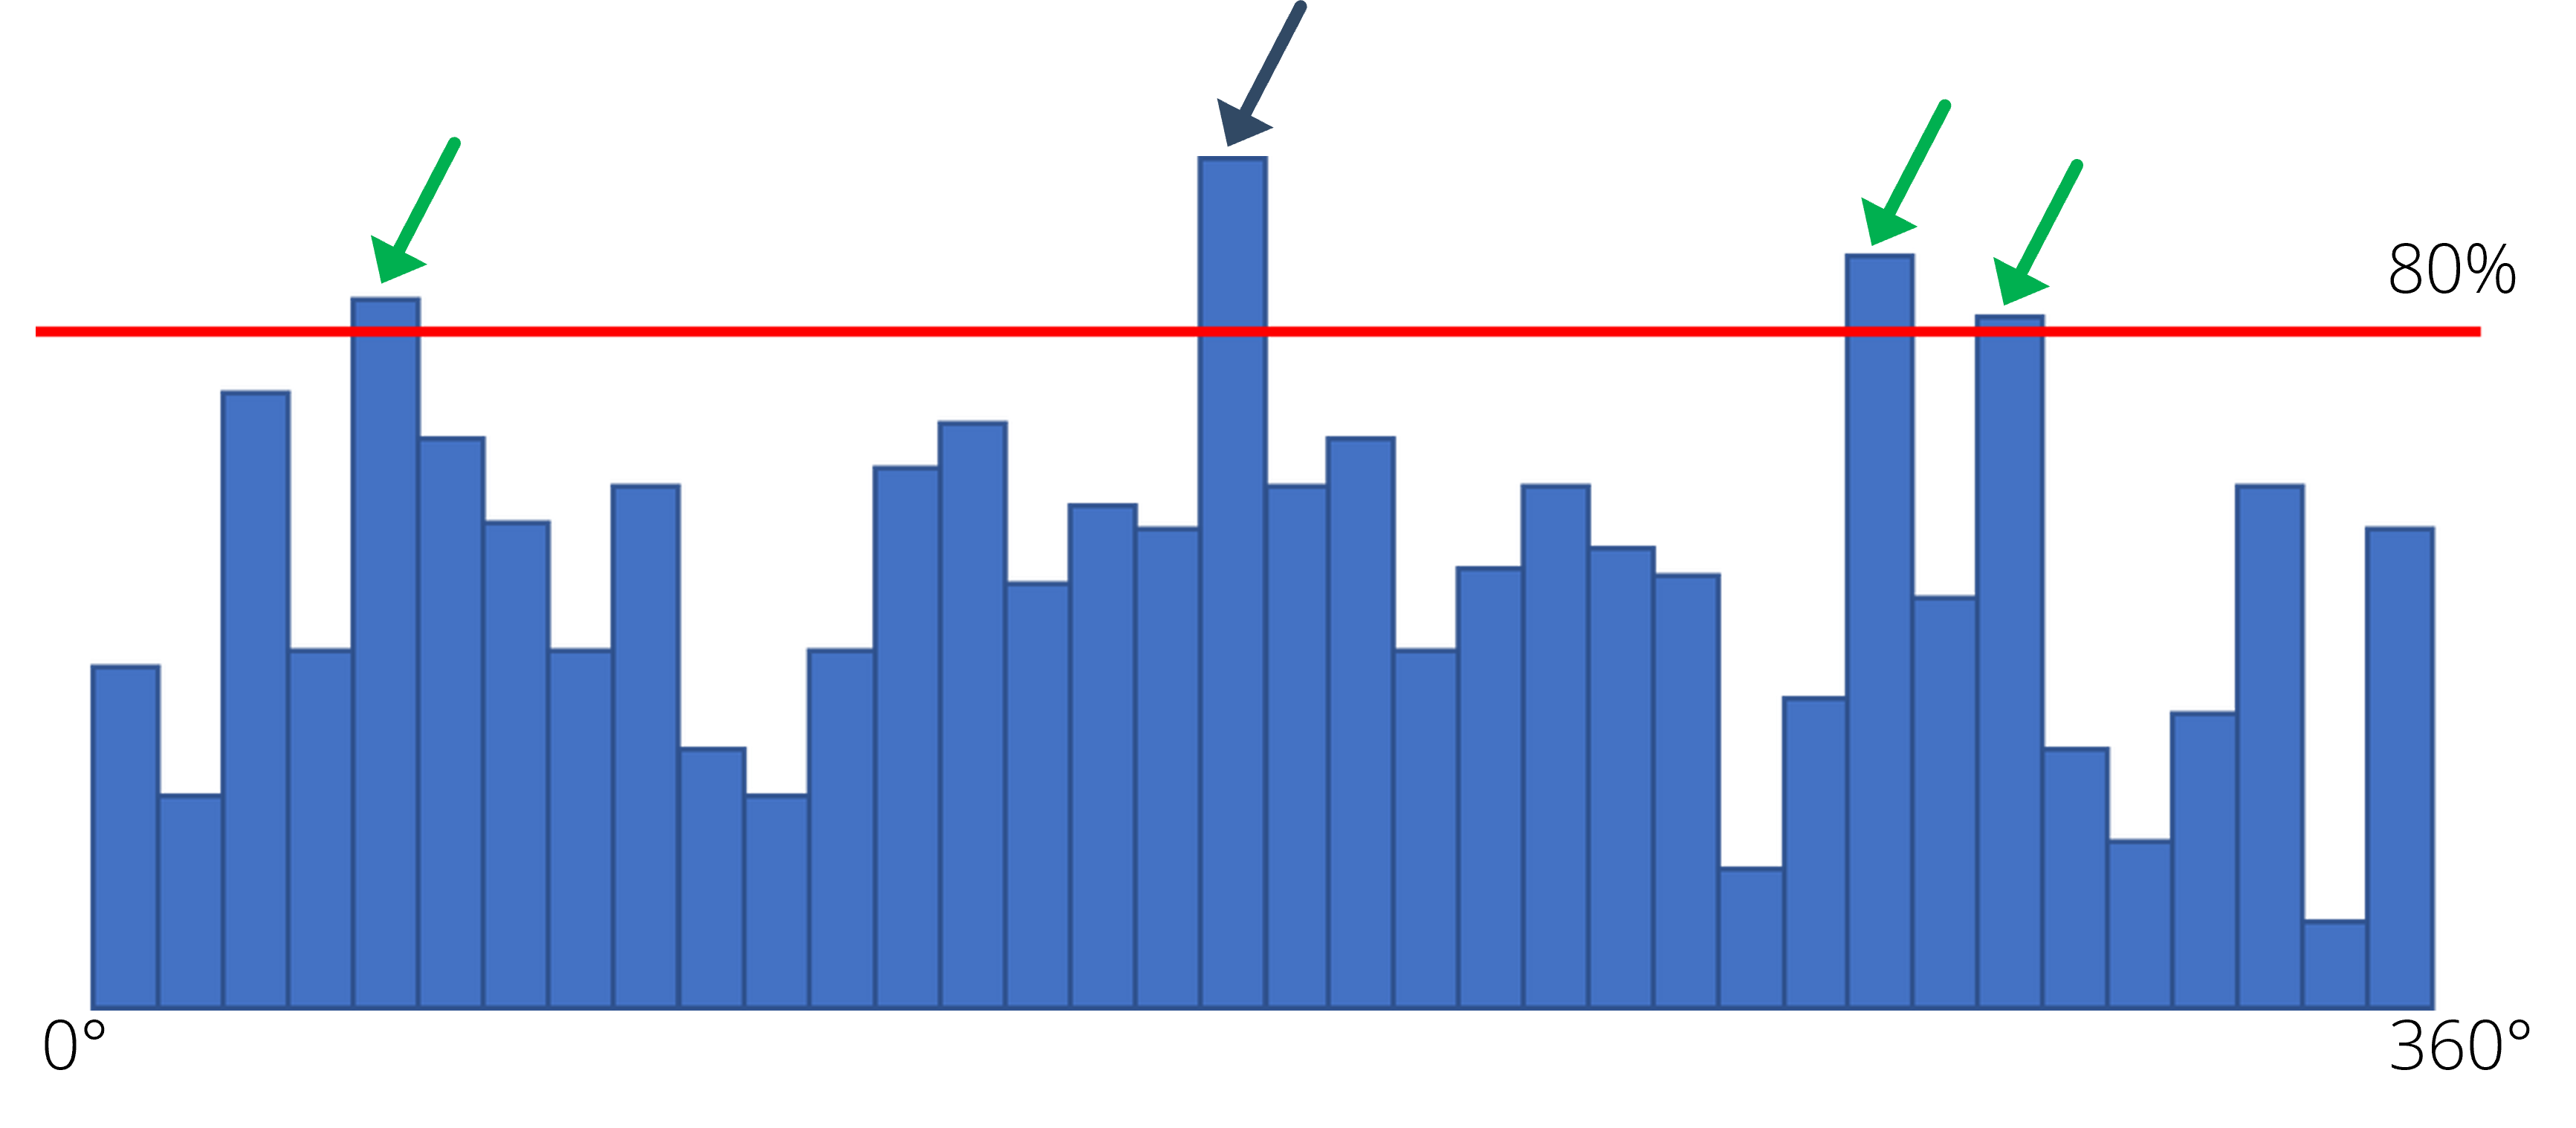
\includegraphics[width=0.8\linewidth]{hist_orientasi.png}
	\caption{Histogram untuk menentukan orientasi dari \textit{keypoint}. Bin dengan nilai tertinggi (tanda panah biru) akan digunakan sebagai orientasi dari \textit{keypoint}. Untuk bin lain yang jumlahnya berada dalam rentang $80\%$ dari bin tertinggi (tanda panah hijau) digunakan untuk membuat \textit{keypoint baru}.}
	\label{fig:hist_orientasi}
\end{figure}

Dari histogram tersebut puncak nilai bin tertinggi akan digunakan sebagai orientasi dari \textit{keypoint}. Untuk puncak-puncak lain yang berada dalam rentang $80\%$ dari puncak tertinggi akan digunakan untuk membuat \textit{keypoint} baru pada lokasi yang sama dengan orientasi yang berbeda sesuai dengan nilai orientasi pada bin tersebut.

\subsection{Pembuatan Deskriptor}
Setelah didapatkan \textit{keypoint} beserta skala dan orientasinya, perlu untuk diberikan sebuah identitas pada setiap \textit{keypoint}. Pemberian identitas ini berguna untuk mengidentifikasi \textit{keypoint} yang satu dengan yang lainnya, agar dapat ditemukan \textit{keypoint-keypoint} dengan ciri yang sama. Identifikasi \textit{keypoint} ditentukan dengan membuat sebuah vektor deskriptor, yaitu vektor yang mendeskripsikan daerah di sekitar \textit{keypoint}. Vektor deskriptor pada SIFT berbentuk vektor sepanjang 128 bilangan bulat.

Pembuatan vektor dilakukan dengan mengambil daerah di sekitar \textit{keypoint} dari gambar yang terlebih dahulu dirotasi sesuai dengan orientasi \textit{keypoint}, ukuran daerah berdasarkan pada skala. Daerah tersebut kemudian dibagi menjadi $4\times4$ subdaerah. Untuk setiap subdaerah dihitung nilai \textit{magnitude} dan orientasi setiap \textit{pixel}-nya dengan diberi bobot menggunakan \textit{Gaussian Weighting} lalu hasilnya dimasukkan ke dalam histogram dengan 8 bin. Setiap bin dalam histogram mewakili 45 derajat orientasi, jumlah dari setiap bin ini akan dijadikan nilai pada vektor deskriptor. Teradapat total 16 subdaerah dengan setiap daerah menghasilkan 8 bilangan, sehingga didapat total sebanyak $16\times8=128$ elemen untuk vektor deskriptor. 

\section{ORB (Oriented FAST and Rotated BRIEF)}
\label{sec:orb}

ORB adalah metode pencarian fitur lokal.

\section{Clustering}
\label{sec:clustering}

\subsection{Agglomerative}
\label{subsec:agglomerative}

\subsection{DBSCAN}
\label{subsec:dbscan}
